%% Submissions for peer-review must enable line-numbering
%% using the lineno option in the \documentclass command.
%%
%% Preprints and camera-ready submissions do not need
%% line numbers, and should have this option removed.
%%
%% Please note that the line numbering option requires
%% version 1.1 or newer of the wlpeerj.cls file, and
%% the corresponding author info requires v1.2

\documentclass[fleqn,10pt]{wlpeerj} % for preprint submissions

% ZNK -- Adding headers for pandoc

\setlength{\emergencystretch}{3em}
\providecommand{\tightlist}{
\setlength{\itemsep}{0pt}\setlength{\parskip}{0pt}}
\usepackage{lipsum}
\usepackage[unicode=true]{hyperref}
\usepackage{longtable}



\usepackage{lipsum} \usepackage{multirow} \usepackage{float}
\floatplacement{figure}{H}

\title{Juvenile Salmon Migration Dynamics in the Discovery Islands and
Johnstone Strait in 2018}

\author[1]{Brett T. Johnson}

\corrauthor[1]{Brett T. Johnson}{\href{mailto:brett.johnson@hakai.org}{\nolinkurl{brett.johnson@hakai.org}}}
\author[]{Julian C.L. Gan}

\author[]{Carly V. Janusson}

\author[1, 2, 3]{Brian P.V. Hunt}


\affil[1]{Hakai Institute Quadra Island Ecological Observatory, Heriot Bay, BC V0P
1H0}
\affil[2]{Institute for the Oceans and Fisheries, University of British Columbia
Vancouver, B.C., Canada V6T 1Z4}
\affil[3]{Department of Earth, Ocean and Atmospheric Sciences, University of
British Columbia Vancouver, B.C., Canada V6T 1Z4}


%
% \author[1]{First Author}
% \author[2]{Second Author}
% \affil[1]{Address of first author}
% \affil[2]{Address of second author}
% \corrauthor[1]{First Author}{f.author@email.com}

% 


\begin{abstract}
The majority of out-migrating juvenile Fraser River salmon
(\emph{Oncorhynchus} spp.) pass northwest through the Strait of Georgia,
the Discovery Islands, and Johnstone Strait. The Discovery Islands to
Johnstone Strait leg of the migration is a region of poor survival for
juvenile salmon relative to the Strait of Georgia. To better understand
the factors that are driving early marine survival through this region
the Hakai Institute Juvenile Salmon Program monitors key aspects of this
migration. Here we report on the 2018 migration in comparison to
averages from the 2015--2018 study period, which we use to define
`normal' in our building time series. In 2018 sockeye (\emph{O. nerka}),
pink (\emph{O. gorbuscha}), and chum (\emph{O. keta}) all migrated
earlier than normal, though not more than by a week. The median capture
date in the Discovery Isalnds was May 23rd for sockeye, five days
earlier than normal; and June 12 for pink and chum, which is five days
earlier for pink and three days earlier than normal for chum. Sea lice
prevalence was lower than normal for sockeye, pink, and chum. Notably,
there were no \emph{Lepeophtheirus salmonis} sea lice observed in
Johnstone Strait in 2018. Sockeye were longer than normal in 2018
whereas pink and chum were smaller than normal. Pink salmon dominated
the catch in 2018, followed by chum, and then socke Sea surface
temperatures in May and June were the warmest on record in the study
period (2015--2018). ye.
% Dummy abstract text. Dummy abstract text. Dummy abstract text. Dummy abstract text. Dummy abstract text. Dummy abstract text. Dummy abstract text. Dummy abstract text. Dummy abstract text. Dummy abstract text. Dummy abstract text.
\end{abstract}

\begin{document}

\flushbottom
\maketitle
\thispagestyle{empty}

\section*{Introduction}\label{introduction}
\addcontentsline{toc}{section}{Introduction}

The first months after marine entry have been identified as a
potentially critical period (R. Beamish and Mahnken 2001) for salmon
stock recruitment, which may ultimately be responsible for inter-annual
variability and long term declines in salmon stocks in British Columbia
(Peterman et al. 2010; R. J. Beamish et al. 2012). Pathogens, parasites,
predators and the impacts of climate change on food web dynamics have
emerged as leading causes for the decline. The Hakai Institute Juvenile
Salmon Program has been monitoring juvenile salmon migrations in the
Discovery Islands and Johnstone Strait (Figure \ref{fig:map}) since 2015
in an effort to understand what factors may be influencing early marine
survival of sockeye, pink, and chum (Hunt et al. 2018). This report
summarizes migration timing, fish length, parasite loads, species
composition, and sea-surface temperature observed from the first 4 years
of this research and monitoring program. These estimates will provide
the context from which to investigate questions and interpret results
related to growth, survival, and the conditions salmon experience during
their migration through this critical region.

\begin{figure}[H]

\includegraphics[width=0.8\linewidth]{map} \hfill{}

\caption{Sampling locations in 2018}\label{fig:map}
\end{figure}

\section*{Methods}\label{methods}
\addcontentsline{toc}{section}{Methods}

\subsection*{Field methods}\label{field-methods}
\addcontentsline{toc}{subsection}{Field methods}

See Hunt et al. (2018) for a detailed description of field and lab
methods. Briefly, we collect juvenile salmon weekly from the Discovery
Islands and Johnstone Strait during their northward migration from the
Strait of Georgia to Queen Charlotte Strait near northern Vancouver
Island, British Columbia. Sampling is conducted from May to July each
year since 2015 using purse seine nets (bunt: 27 m x 9 m with 13 mm
mesh; tow: 46 m x 9 m with 76 mm mesh). We sample in nearshore marine
habitats with depth \textgreater{} 10 m and effectively sample sockeye
(\emph{Oncorhynchus nerka}), pink (\emph{O. gorbuscha}), chum (\emph{O.
keta}) and incidentally capture coho (\emph{O. kisutch}), chinook
(\emph{O. tshawytschya}) and Pacific herring (\emph{Clupea pallasii}).
All animal care was in accordance with Animal Care Guidelines under
permit A16-0101. Temperature data were collected by deploying an RBR
conductivity, temperature, and depth profiler to depths \textgreater{}
30 m at station QU39 (Figure \ref{fig:map}) in the northern Strait of
Georgia.

\subsection*{Statistical methods}\label{statistical-methods}
\addcontentsline{toc}{subsection}{Statistical methods}

All metrics reported are in relation to the time series average
(2015-2018). The mean for each parameter of interest was calculated for
all years combined, and the z-score was calculated for each parameter to
determine the number of standard deviations away from the mean a given
parameter was in each year.

The peak migration date for each species was estimated by calculating
the median date of capture in the Discovery Islands---the date at which
50 percent of the fish passed through the region. Because very few pink
are caught in odd years, only even years were included in the
calculation of the time serie average. To visualize migration timing we
plotted cumulative catch abundance between May 1st and July 9th each
year and fit a logistic growth line. Species proportions were calculated
by dividing the total number of each species caught, by the sum of all
species caught that season. Only seines that contained sockeye were used
in the calculation of species proportions, so in effect this species
proportion measure is representative of the salmon community composition
that co-migrate with sockeye. Fork length distributions were visualized
by calculating kernel density estimates from fork length data. The
prevalence, intensity, and abundance of sealice was calculated as
detailed in Margolis et al. (1990). The mean sea surface temperature was
calculated from the top 30 m of the water column in May and June from
all years. To visualize temperature anomalies we applied a loess
regression to sea surface temperatures from all four years to develop a
model that would represent the seasonal trend.

\section*{Results and Discussion}\label{results-and-discussion}
\addcontentsline{toc}{section}{Results and Discussion}

\subsection*{Migration Timing}\label{migration-timing}
\addcontentsline{toc}{subsection}{Migration Timing}

Migration timing in the Discovery Islands in 2018 did not differ from
the time series average by more than a week for sockeye, pink, or chum.
The peak migration date for sockeye in the Discovery Islands was on May
23, 5 days earlier than average of May 28 (z-score = -0.71) (Figure
\ref{fig:mt}). The peak migration date for pink in the Discovery Islands
was on June 12, 5.25 days earlier than average of June 17 (z-score =
-0.38). The peak migration date for chum in the Discovery Islands was on
June 12, 2.5 days earlier than average of June 14 (z-score = -0.29).

\begin{figure}[H]
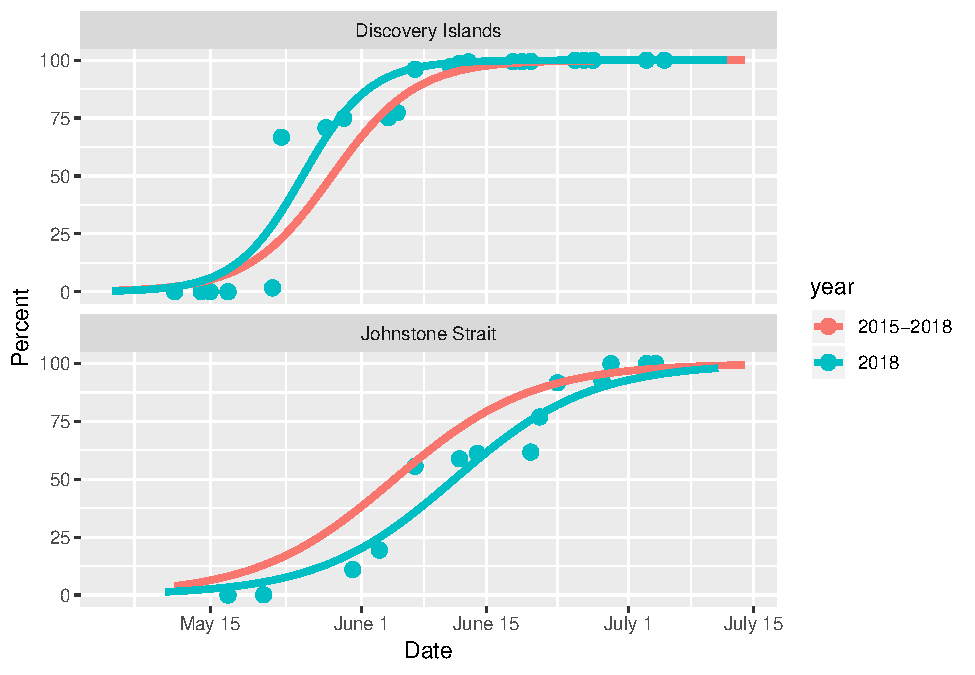
\includegraphics[width=0.8\linewidth]{peer_j_migration_dynamics_files/figure-latex/mt-1} \caption{Cumulative catch of juvenile sockeye salmon migrating through the Discovery Islands compared to the average for 2015--2018. Migration curves were predicted by fitting a logistic growth equation to the cumulative percent of sockeye in each year.}\label{fig:mt}
\end{figure}

\begin{longtable}[]{@{}llrrr@{}}
\caption{\label{tab:mtdi} Migration timing statistics for the cumulative
catch of sockeye, pink, and chum salmon in the Discovery Islands in
2018, compared to the time-series average.}\tabularnewline
\toprule
Species & Year & Q1 & Peak Date & Q3\tabularnewline
\midrule
\endfirsthead
\toprule
Species & Year & Q1 & Peak Date & Q3\tabularnewline
\midrule
\endhead
Sockeye & Average & May 26 & May 28 & June 04\tabularnewline
~ & 2018 & May 23 & May 23 & June 04\tabularnewline
Pink & Average & June 06 & June 17 & June 22\tabularnewline
~ & 2018 & June 07 & June 12 & June 12\tabularnewline
Chum & Average & June 06 & June 14 & June 22\tabularnewline
~ & 2018 & June 07 & June 12 & June 20\tabularnewline
\bottomrule
\end{longtable}

\subsection*{Length}\label{length}
\addcontentsline{toc}{subsection}{Length}

Fish lengths varied between regions, species and year (Figure
\ref{fig:length}). In 2018 Sockeye lengths were on average 116.9 mm,
which is 8.9 mm longer than average (\emph{p} \textless{} 0.0001, 95\%
CI 6.2, 11.7). Pink lengths were on average 96.3 mm, which is 8.8 mm
shorter than average (\emph{p} \textless{} 0.0001, 95\% CI 10.9, 6.7).
Chum were on average 103.4 mm, which is 7 mm shorter than average
(\emph{p} \textless{} 0.0001, 95\% CI 8.9, 5).

\begin{figure}[H]
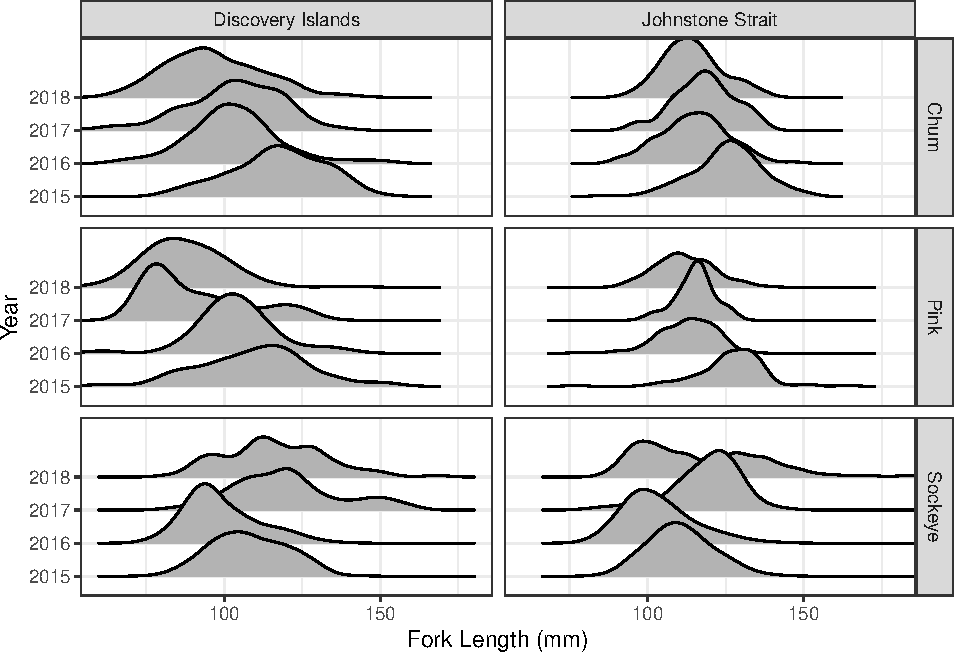
\includegraphics[width=0.8\linewidth]{peer_j_migration_dynamics_files/figure-latex/length-1} \caption{Kernel density distributions of juvenile salmon fork lengths for each year in the selected region. Note that these distributions contain multiple age-classes.}\label{fig:length}
\end{figure}

\subsection*{Species Proportions}\label{species-proportions}
\addcontentsline{toc}{subsection}{Species Proportions}

Pink salmon dominated the catch in the Discovery Islands and Johnstone
Strait in 2018 making up 51.9 percent of the catch while chum made up
32.4 percent and sockeye 12.9 (Figure \ref{fig:prop}).

\begin{figure}[H]
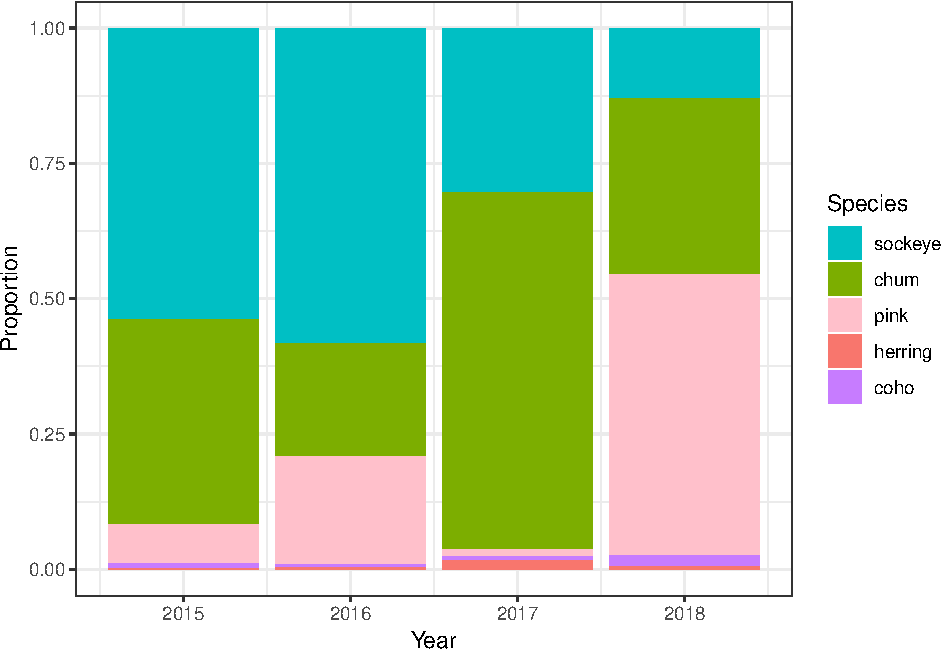
\includegraphics[width=0.8\linewidth]{peer_j_migration_dynamics_files/figure-latex/prop-1} \caption{The annual proportion of fish captured in the Discovery Islands and Johnstone Strait combined.}\label{fig:prop}
\end{figure}

\subsection*{Parasite Loads}\label{parasite-loads}
\addcontentsline{toc}{subsection}{Parasite Loads}

\begin{verbatim}
## [1]  1.36612945 -0.42022364  0.03189039 -0.97779620
\end{verbatim}

Across the Discovery Islands and Johnstone Strait, parasite loads were
11.8 percent less than average (Z = -0.98) The prevalence of motile
(pre-adult and adult life stage) sea lice in 2018 was the lowest
recorded in the time-series (Figure \ref{fig:sealice}). Notably, no
\emph{Lepeophtheirus salmonis} were detected on sockeye in Johnstone
Strait, despite being present in the Discovery Islands. Pink salmon
appeared to have higher counts of \emph{Caligus clemensi} in 2018
compared to chum and sockeye.

\begin{figure}[H]
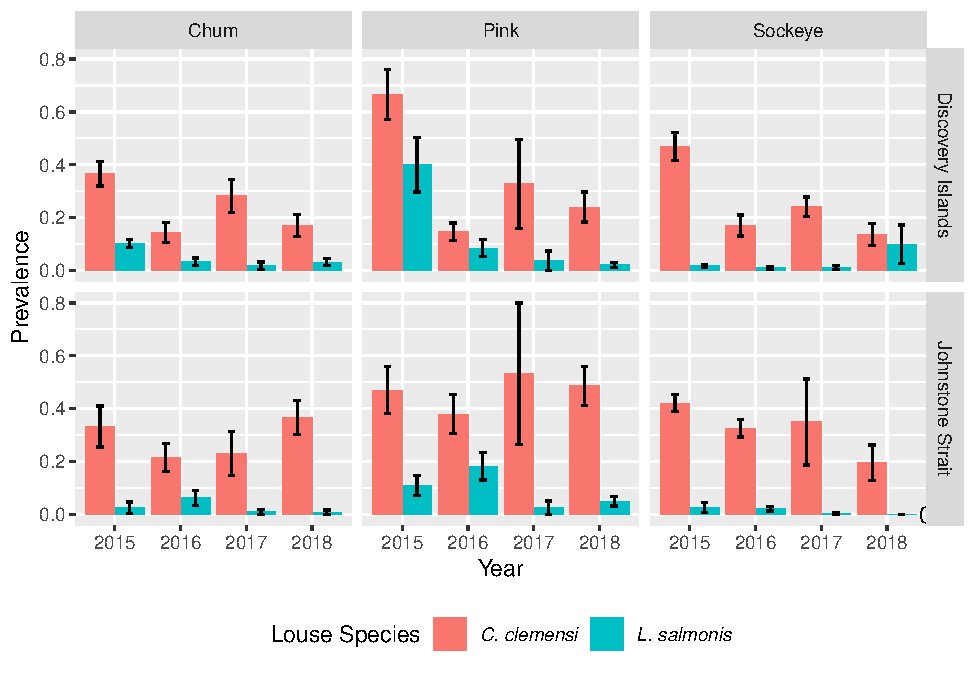
\includegraphics[width=0.8\linewidth]{peer_j_migration_dynamics_files/figure-latex/sealice-1} \caption{The prevalence (+/-SE) of motile sea lice on juvenile salmon in the Discovery Islands and Johnstone Strait.}\label{fig:sealice}
\end{figure}

\subsection*{Sea Surface Temperature}\label{sea-surface-temperature}
\addcontentsline{toc}{subsection}{Sea Surface Temperature}

Sea-surface temperatures in May and June at QU39 in the northern Strait
of Georgia was 0.39 degrees C warmer than normal (Z = 1.33). Sea surface
temperatures between May and July of 2018 were warmer than the time
series average. (Figure \ref{fig:sst})

\begin{figure}[H]
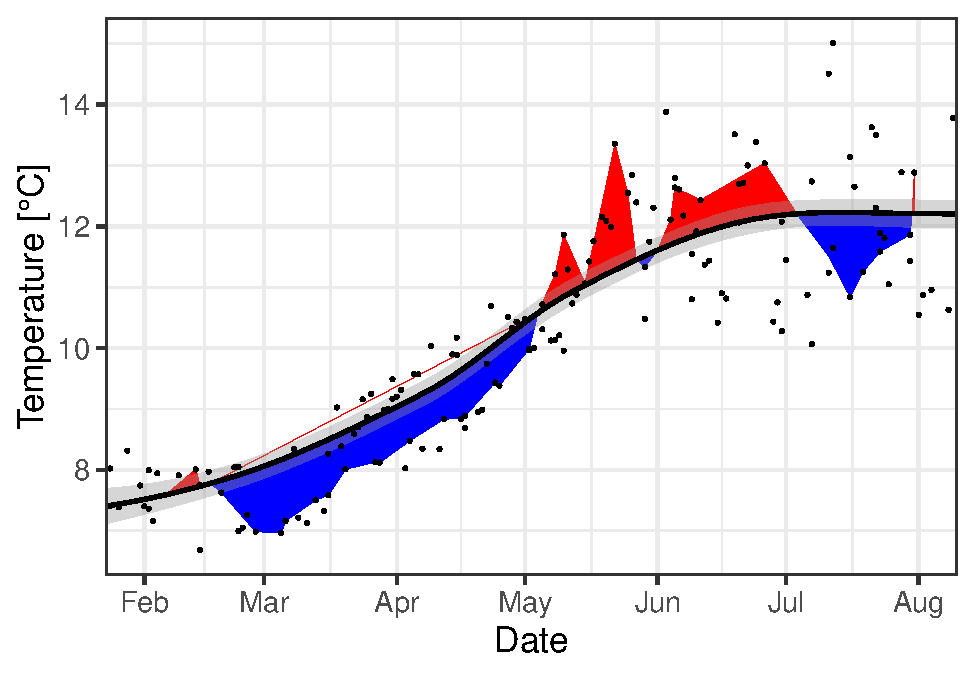
\includegraphics[width=0.8\linewidth]{peer_j_migration_dynamics_files/figure-latex/sst-1} \caption{Time series of 30 m depth integrated temperature anomalies observed at Hakai Oceanographic Monitoring station QU39. Blue areas represent temperatures that are below normal, red areas represent above normal temperatures at the selected station in 2018. Normal is the solid black line which is a loess regression based on temperatures from 2015-2018. The shaded grey area is 1 SE of the loess regression. The black dots are the daily minimum and maximum temperatures observed over the time series.}\label{fig:sst}
\end{figure}

\section*{References}\label{references}
\addcontentsline{toc}{section}{References}

\hypertarget{refs}{}
\hypertarget{ref-Beamish2012}{}
Beamish, R. J., C. Neville, R. Sweeting, and K. Lange. 2012. ``The
synchronous failure of juvenile pacific salmon and herring production in
the strait of georgia in 2007 and the poor return of sockeye salmon to
the Fraser river in 2009.'' \emph{Marine and Coastal Fisheries} 4 (1):
403--14.
doi:\href{https://doi.org/10.1080/19425120.2012.676607}{10.1080/19425120.2012.676607}.

\hypertarget{ref-Beamish2001}{}
Beamish, RJ, and Conrad Mahnken. 2001. ``A critical size and period
hypothesis to explain natural regulation of salmon abundance and the
linkage to climate and climate change.'' \emph{Progress in Oceanography}
49: 423--37.

\hypertarget{ref-Hunt2018}{}
Hunt, Brian P.V., Brett T. Johnson, Sean C. Godwin, Martin Krkošek,
Evgeny A Pakhomov, and Luke A Rogers. 2018. ``The Hakai Institute
Juvenile Salmon Program : Early Life History Drivers of Marine Survival
in Sockeye , Pink and Chum Salmon in British Columbia.'' Institute for
the Oceans; Fisheries; Department of Earth, Ocean; Atmospheric Sciences,
University of British Columbia, Hakai Institute, Earth to Ocean Research
Group, Simon Fraser University, Department of Ecology; Evolutionary
Biology, Univer.

\hypertarget{ref-Margolis1990}{}
Margolis, L., G. W. Esch, A.M. Kuris, and G.A. Schad. 1990. ``The Use of
Ecological Terms in Parasitology (Report of an Ad Hoc Committee of the
American Society of Parasitologists).'' \emph{The Journal of
Parisitology} 68 (1): 131--33.
doi:\href{https://doi.org/10.2307/3281335}{10.2307/3281335}.

\hypertarget{ref-Peterman2010}{}
Peterman, Randall M, D Marmorek, B Beckman, M Bradford, M Lapointe, N
Mantua, Brian Riddell, et al. 2010. ``Synthesis of evidence from a
workshop on the decline of Fraser River sockeye. June 15-17, 2010. A
Report to the Pacific Salmon Commission.'' August. Vancovuer, British
Columbia: Pacific Salmon Commission.



\end{document}
